% ------------------------------------------------------------------------------
% CHAPTER 2: PAPER 1 (AAS 25-787)
% ------------------------------------------------------------------------------
\chapter{Advanced Modeling Techniques for Analyzing Space Debris Fragmentation and Evolution}
\chaptermark{Symplectic Debris Fragmentation Modeling}
\label{ch:paper1}

\section*{Chapter Overview and Contextualization}
This chapter addresses the first specific objective of this doctoral research by developing and validating a structure-preserving $N$-body propagation framework for high-density space debris environments. This chapter synthesizes and presents the research published in the \textit{AAS/AIAA Astrodynamics Specialist Conference} (Paper AAS 25-787).

Predicting the evolutionary trajectory of fragmentation clouds requires maintaining numerical stability across millions of integration steps. Traditional explicit numerical propagators (e.g., standard Runge-Kutta or Cowell formulations) suffer from the accumulation of truncation errors, which manifest as non-physical secular drifts in mechanical energy. This chapter evaluates the application of symplectic integration schemes---specifically the WHFast symplectic $N$-body solver from the REBOUND library---to model the motion of 20,000 autonomous fragments under Earth's central gravity and zonal geopotential harmonics ($J_2$ and $J_4$).

The primary contribution of this work lies in proving that symplectic $N$-body formulations maintain bounded relative energy errors ($|\Delta E/E_0| \le 10^{-7}$) over extended propagation windows while delivering sub-kilometer orbital element consistency when benchmarked against NASA's General Mission Analysis Tool (GMAT). Furthermore, computational scalability tests demonstrate that the architecture follows a predictable power-law scaling exponent of 1.60, establishing the numerical baseline required for the subsequent integration of dissipative environmental perturbations.

\newpage
% \includepdf[pages=-, scale=0.95, pagecommand={\thispagestyle{plain}}]{papers/AAS_25_787.pdf}

\clearpage

% Check if the compiled PDF exists; embed if found, display placeholder if missing
\IfFileExists{papers/paper1.pdf}{%
    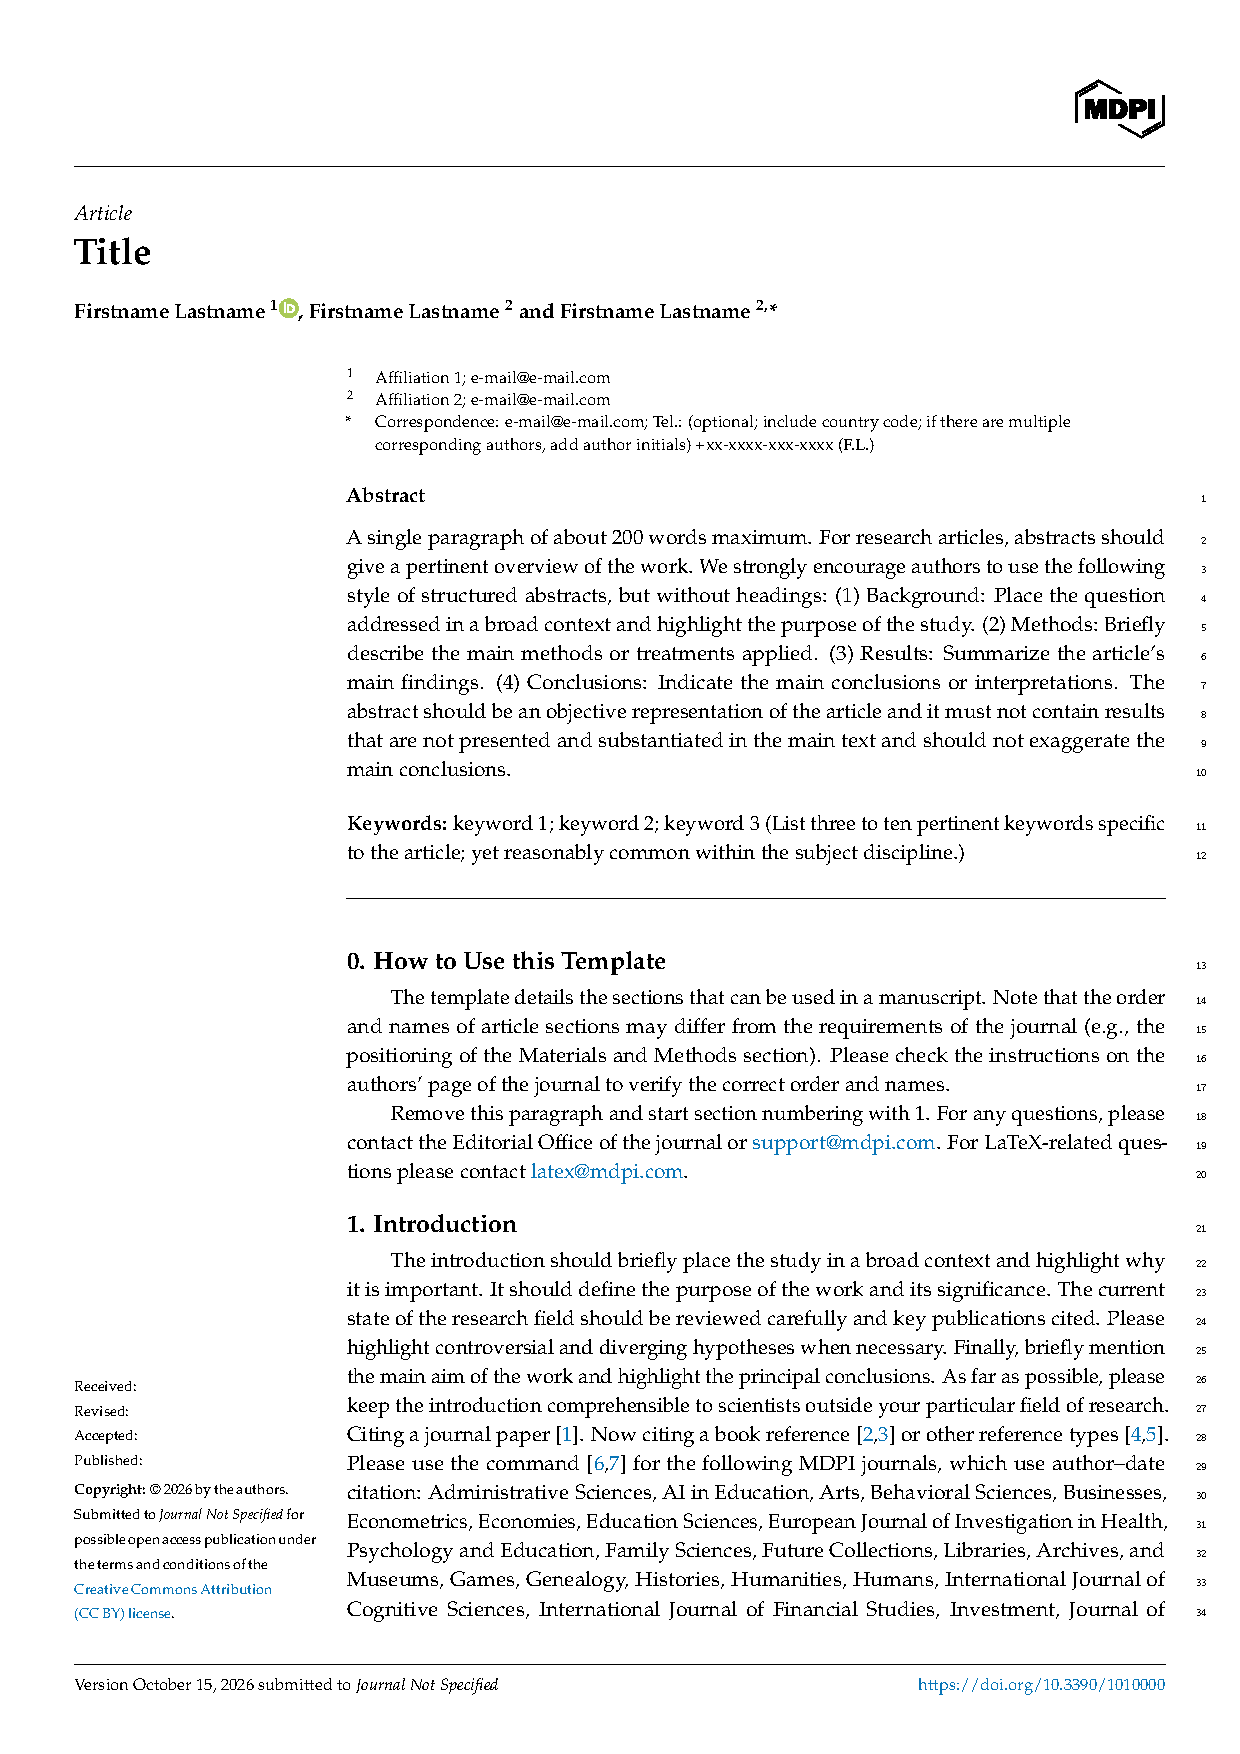
\includepdf[
        pages=-,
        scale=0.95,
        pagecommand={\thispagestyle{plain}}
    ]{papers/paper1.pdf}%
}{%
    \vspace*{2cm}
    \begin{center}
        \fbox{%
            \begin{minipage}{0.85\textwidth}
                \centering\vspace{1cm}
                \textbf{\large [Paper 1 PDF Pending: \texttt{papers/paper1.pdf}]}\\[0.5cm]
                \textit{The compiled PDF was not found in the \texttt{papers/} directory.}\\
                Link or upload the compiled PDF as \texttt{papers/paper1.pdf} to embed the complete publication.
                \vspace{1cm}
            \end{minipage}%
        }
    \end{center}
}